\documentclass{article}
\usepackage{CJK}
\usepackage{amsmath,amssymb}
\usepackage{geometry,graphicx}
\geometry{bottom = 3cm, left = 3cm, right = 3cm, top = 3cm}
\title{数值代数说明文档}
\author{张奇 PB19000093}
\begin{document}
\begin{CJK}{UTF8}{gbsn}
    	\maketitle
    \section{实验内容}
    	本次实验对于三种情况实现Richardson外推法的数值导数,如下
    	\begin{itemize}
    		\item $\log(x), x=3, M=3.$
    		\item $\tan(x), x=\sin^{-1}0.8, M=4.$
    		\item $\sin(x^2+\frac{x}{3}), x=0, M=5.$
    	\end{itemize}
    	其中$M$代表外推的次数,最终将外推的结果以三角形金字塔的方式输出。
    \section{算法实现}
    	实验在数值上容易实现,首先考虑二阶近似
    	\[ \dfrac{f(x+h) - f(x-h)}{2h} = f'(x) - \sum_{i=1} a_{2i-1} h^{2i-1},\]
    	其中 $a_{2i-1} = \dfrac{2f^{2i-1}(x)}{(2i-1)!},$ 由泰勒展开得到。
    	为了消去余项,考虑记$D(n,0) = \dfrac{f(x+h/2^n) - f(x-h/2^n)}{2h/2^n},$用递推公式
    	$D(j,k+1) = \dfrac{4^{k+1} D(j+1,k) - D(j,k) }{4^{k+1} - 1},$每次提高两个精度。
    	最终输出并且比较误差。
    	\section{编译环境}
    	\begin{itemize}
    		\item 编译器:g++ (Ubuntu 9.4.0-1ubuntu1~20.04.1) 9.4.0.
    		\item 编译命令:./run  lab6
    	\end{itemize}
    \section{结果总结}
    \begin{figure}[hbpt]
    	\centering
    	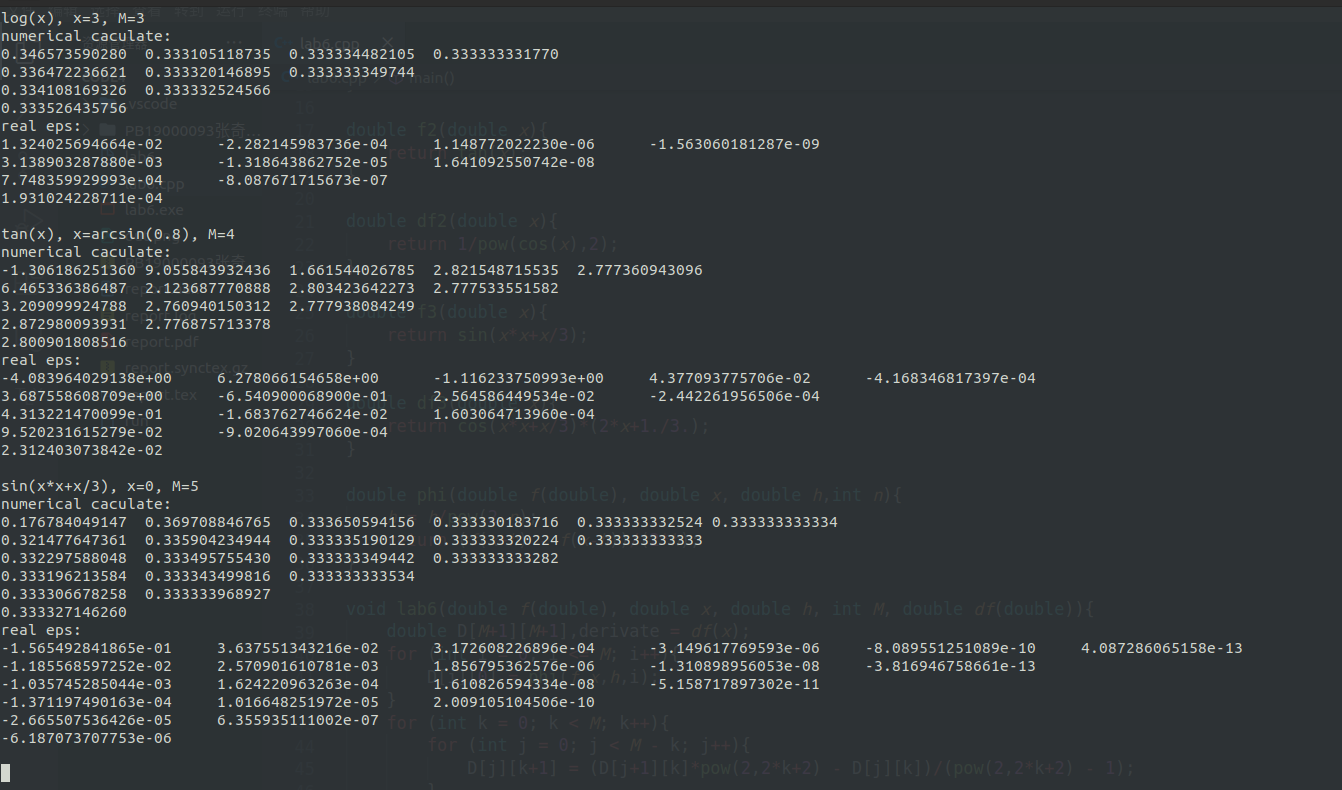
\includegraphics[width=8cm]{./code4.png}
    	\caption{实验结果}
    \end{figure}
    \paragraph{分析}
  	在第三个函数的导数处一定要注意$1/3=0,1./3.=0.33333$。
\end{CJK}
\end{document}